\section{Tabelle complete di convergenza e diagnostiche MMS}
\label{app:mms}

\subsection{Raffinamento spaziale}

La Tabella~\ref{tab:spatial-full} riporta gli errori $L^2$ e $H^1$ della serie coordinata. Lo spostamento è approssimato con elementi quadratici, mentre pressione e tracciante usano elementi lineari. Il tasso $H^1$ del tracciante non risulta ancora stabilizzato; inoltre, il raffinamento temporale coordinato con quello spaziale implica che gli EOC osservati non isolano completamente l'errore spaziale.

\begin{table*}[!t]
\centering
\caption{Errori MMS spaziali completi. Gli EOC sono calcolati tra livelli consecutivi; $h=1/N$ indica la larghezza della cella quadrata.}
\label{tab:spatial-full}
\scriptsize
\begin{tabular}{c|cc|cc|cc}
\toprule
$h=1/N$ & $\|e_d\|_{L^2}$ & $\|e_d\|_{H^1}$ & $\|e_p\|_{L^2}$ & $\|e_p\|_{H^1}$ & $\|e_c\|_{L^2}$ & $\|e_c\|_{H^1}$\\
\midrule
0.2500 & $2.6870\cdot10^{-3}$ & $7.2341\cdot10^{-2}$ & $5.4526\cdot10^{-3}$ & $1.2690\cdot10^{-1}$ & $2.4562\cdot10^{-2}$ & $1.2535\cdot10^{-1}$\\
0.1250 & $3.5294\cdot10^{-4}$ & $1.8383\cdot10^{-2}$ & $1.3055\cdot10^{-3}$ & $6.3093\cdot10^{-2}$ & $6.3959\cdot10^{-3}$ & $3.8283\cdot10^{-2}$\\
0.0625 & $4.4932\cdot10^{-5}$ & $4.6130\cdot10^{-3}$ & $3.2286\cdot10^{-4}$ & $3.1496\cdot10^{-2}$ & $1.6164\cdot10^{-3}$ & $1.4518\cdot10^{-2}$\\
\midrule
EOC $0.25\to0.125$ & 2.93 & 1.98 & 2.06 & 1.01 & 1.94 & 1.71\\
EOC $0.125\to0.0625$ & 2.97 & 1.99 & 2.02 & 1.00 & 1.98 & 1.40\\
\bottomrule
\end{tabular}
\end{table*}
\FloatBarrier

\subsection{Raffinamento temporale e bilanci}

\begin{table*}[!t]
\centering
\caption{Errori $L^2$ e tassi temporali osservati con spazio FEM fissato $Q_2/Q_2/Q_2$.}
\label{tab:temporal-full}
\small
\begin{tabular}{c|cc|cc|cc}
\toprule
$\Delta t_{\max}$ & $\|e_d\|_{L^2}$ & EOC$_t$ & $\|e_p\|_{L^2}$ & EOC$_t$ & $\|e_c\|_{L^2}$ & EOC$_t$\\
\midrule
0.05000 & $1.3569\cdot10^{-3}$ & -- & $2.7205\cdot10^{-2}$ & -- & $1.3713\cdot10^{-1}$ & --\\
0.02500 & $6.3341\cdot10^{-4}$ & 1.10 & $1.3843\cdot10^{-2}$ & 0.97 & $7.0004\cdot10^{-2}$ & 0.97\\
0.01250 & $3.0010\cdot10^{-4}$ & 1.08 & $6.9863\cdot10^{-3}$ & 0.99 & $3.5421\cdot10^{-2}$ & 0.98\\
0.00625 & $1.4436\cdot10^{-4}$ & 1.06 & $3.5106\cdot10^{-3}$ & 0.99 & $1.7835\cdot10^{-2}$ & 0.99\\
\bottomrule
\end{tabular}
\end{table*}
\FloatBarrier

\begin{table}[!htbp]
\centering
\caption{Residuo energetico cumulativo finale al variare del passo massimo sul dominio unitario.}
\label{tab:energy-dt}
\small
\begin{tabular}{cc}
\toprule
$\Delta t$ & $|R_N|$\\
\midrule
0.040 & $2.0739\cdot10^{-3}$\\
0.020 & $1.1042\cdot10^{-3}$\\
0.010 & $5.7074\cdot10^{-4}$\\
0.005 & $2.9028\cdot10^{-4}$\\
\bottomrule
\end{tabular}
\end{table}
\FloatBarrier

La massa passa da $M(0)=0.1628317137332642$ a $M(T)=0.1628317137332636$, con drift relativo $3.92\times10^{-15}$. Il residuo di compatibilità iniziale è $5.45\times10^{-16}$ e l'errore massimo dell'identità algebrica al passo è $4.78\times10^{-17}$. Tali valori descrivono i casi eseguiti e non costituiscono una dimostrazione generale della stabilità energetica dello schema discreto.

\begin{figure*}[!t]
\centering
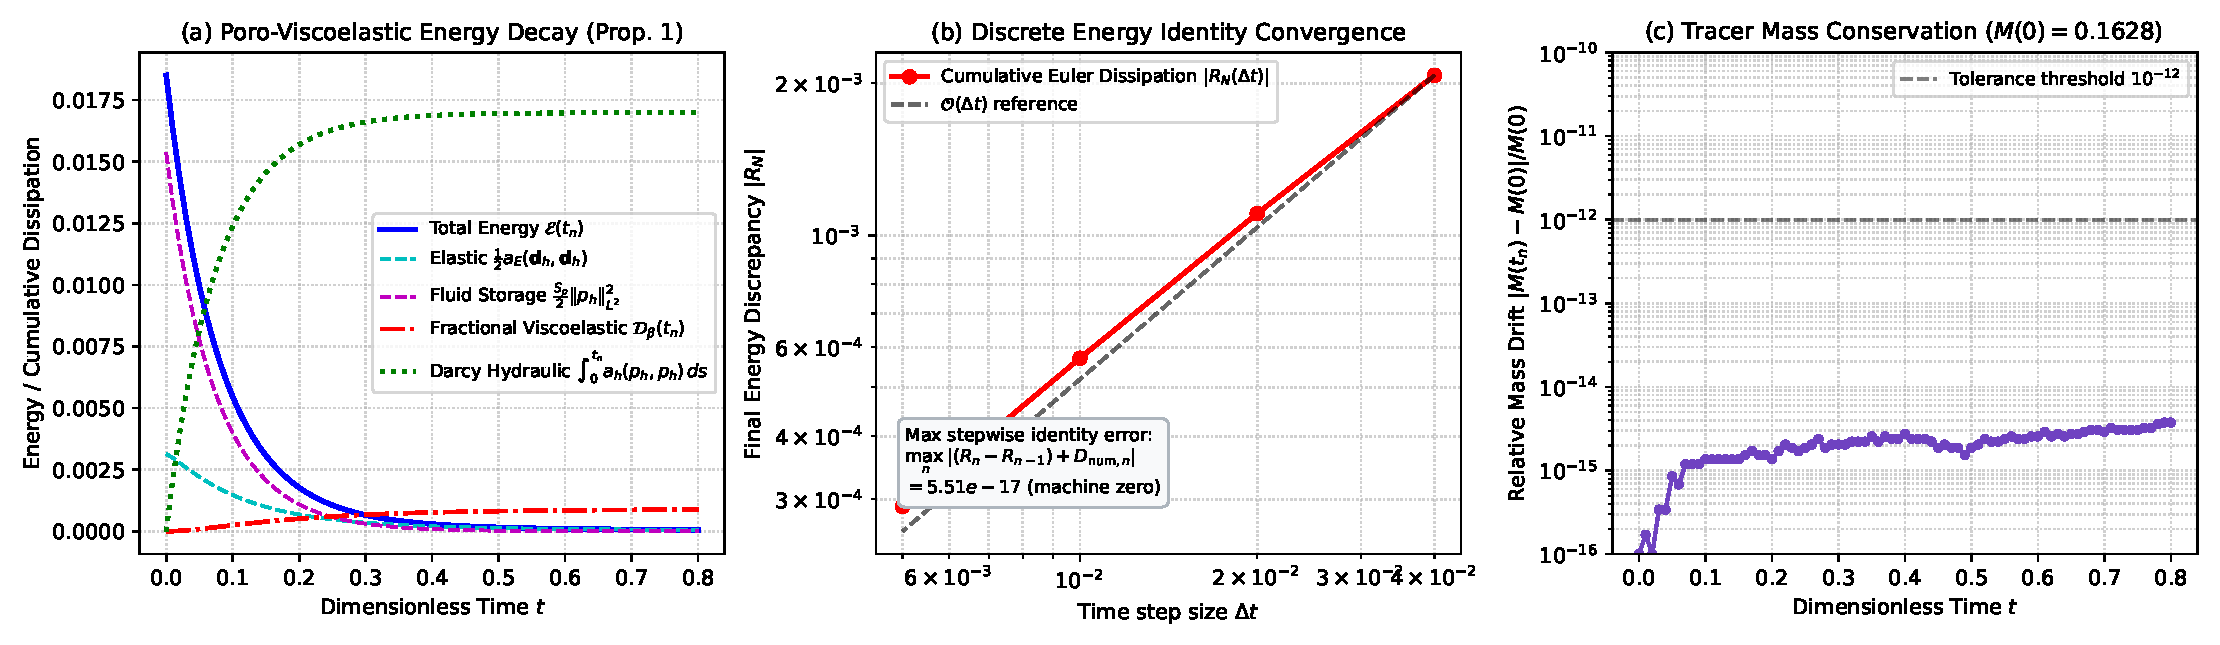
\includegraphics[width=0.78\textwidth]{appendices/figs_01_energy_and_mass_conservation.pdf}
\caption{Diagnostiche di energia e massa sul dominio MMS unitario. Questa prova è distinta dal caso anatomico forzato.}
\label{fig:app-mms-energy}
\end{figure*}

\begin{figure*}[!t]
\centering
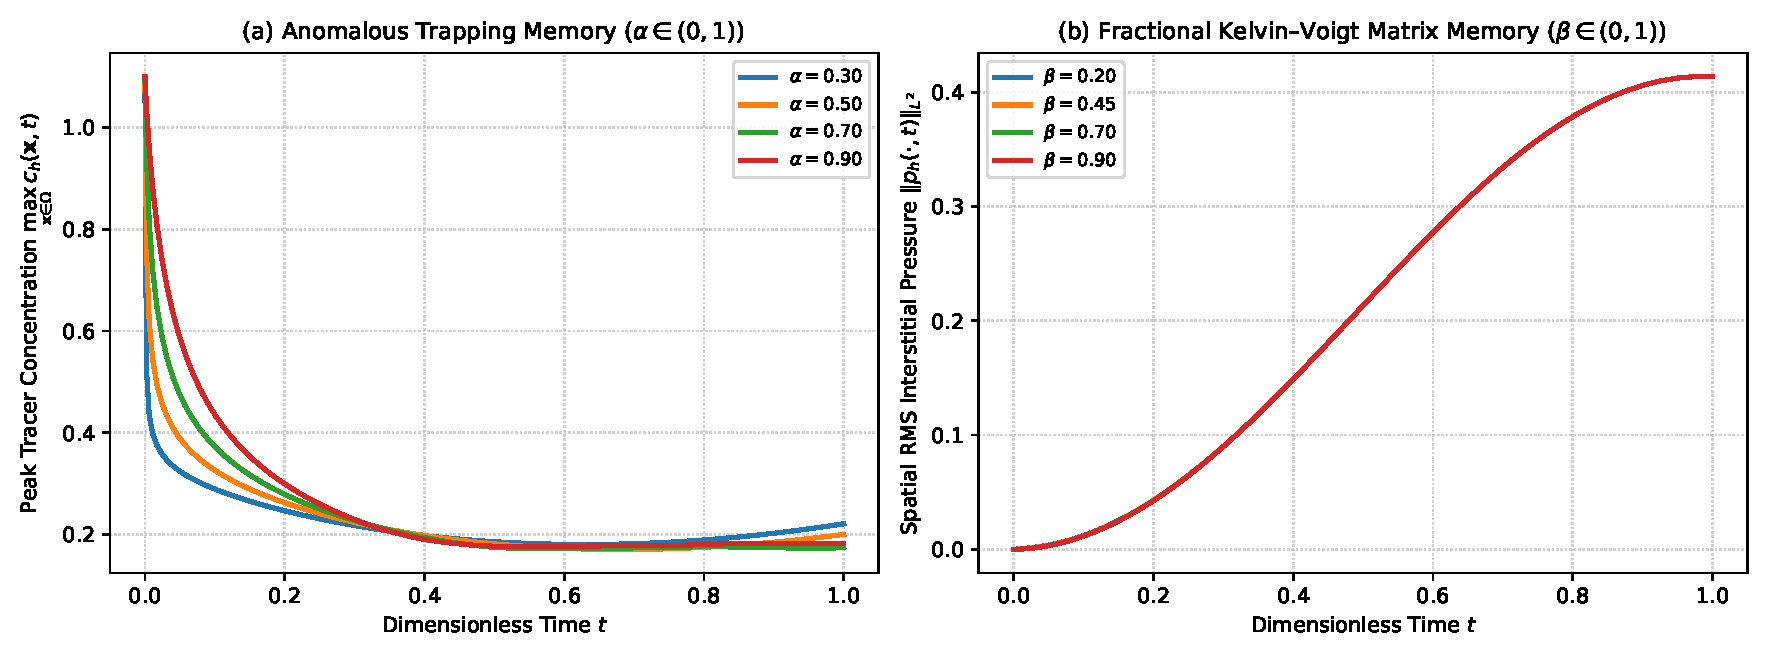
\includegraphics[width=0.78\textwidth]{appendices/figs_02_fractional_orders_physics_sensitivity.pdf}
\caption{Sensibilità delle traiettorie agli ordini frazionari sul dominio unitario. Il grafico è diagnostico e non dimostra, da solo, identificabilità dei parametri.}
\label{fig:app-mms-fractional}
\end{figure*}
